\subsubsection{Missing Values}\label{sssec:missingvalues}
It was known that the dataset contained some missing values, so further analysis was conducted on each feature to identify these missing values. A python script called \textbf{dataexp.py} was created to analyse these features. First off, the whole dataset was checked to see what would happen if the instances with missing values were to be removed. In Table \ref{table:miss_val} it is shown that there would be too much data loss if these instances were to be dropped (around 50\% would be lost). 

\begin{table}[H]
\centering
\begin{tabular}{|c|c|c|c|c|}
\hline
\textbf{Year} & \textbf{Total Instances} & \textbf{Missing Values} & \textbf{No  Missing Values} & \textbf{Data Loss} \\ \hline
1\_year       & 7027                     & 3833                    & 3194                        & 0.5455             \\ \hline
2\_year       & 10173                    & 6085                    & 4088                        & 0.5982             \\ \hline
3\_year       & 10503                    & 5618                    & 4885                        & 0.5349             \\ \hline
4\_year       & 9792                     & 5023                    & 4769                        & 0.5130             \\ \hline
5\_year       & 5910                     & 2879                    & 3031                        & 0.4871             \\ \hline
\end{tabular}
\caption{Missing values stats, output generated using \textbf{dataexp.py}}
\label{table:miss_val}
\end{table}

\noindent Furthermore, another third party library called \textbf{missinggo} \cite{python:missinggo} was used to further help us analyse/visualize these features with missing values. The nullity matrix in this library was used to find patterns visually for missing values. As shown in Figure \ref{fig:nullity_matrix} features \textbf{X21} and \textbf{X37} have the most missing values in 'Year 2'. 

\begin{figure}[H]
\centering
  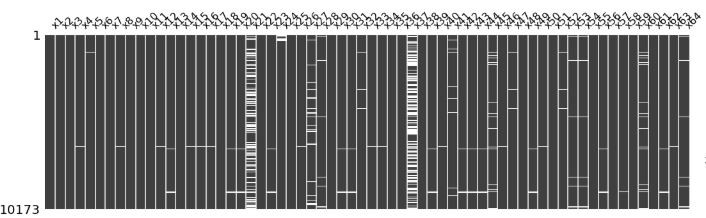
\includegraphics[scale = .78]{imgs/nullity_matrix.JPG}
  \caption{ Nullity Matrix for Year 2. White space means missing values for the specific feature. }
  \label{fig:nullity_matrix}
\end{figure}

\noindent The nullity matrix plots were generated for each forecasting period/year. Another plot which was used from this library is called the correlation heatmap which measures the nullity correlation between the features. This helped to identify the correlation of nullity between each feature, meaning if a value of 1 is shown in the box, it means that if one feature is missing the other is also missing. On the other hand if -1 is shown it means if one feature is missing the other is not. The output can be a value between -1 to 1 and if the value is to small (-0.05 < V < 0.05), nothing is shown. Again these plots where generated for all forecasting periods/years. An example for this plot is shown in Figure \ref{fig:nullity_heatmap}.

\begin{figure}[H]
\centering
  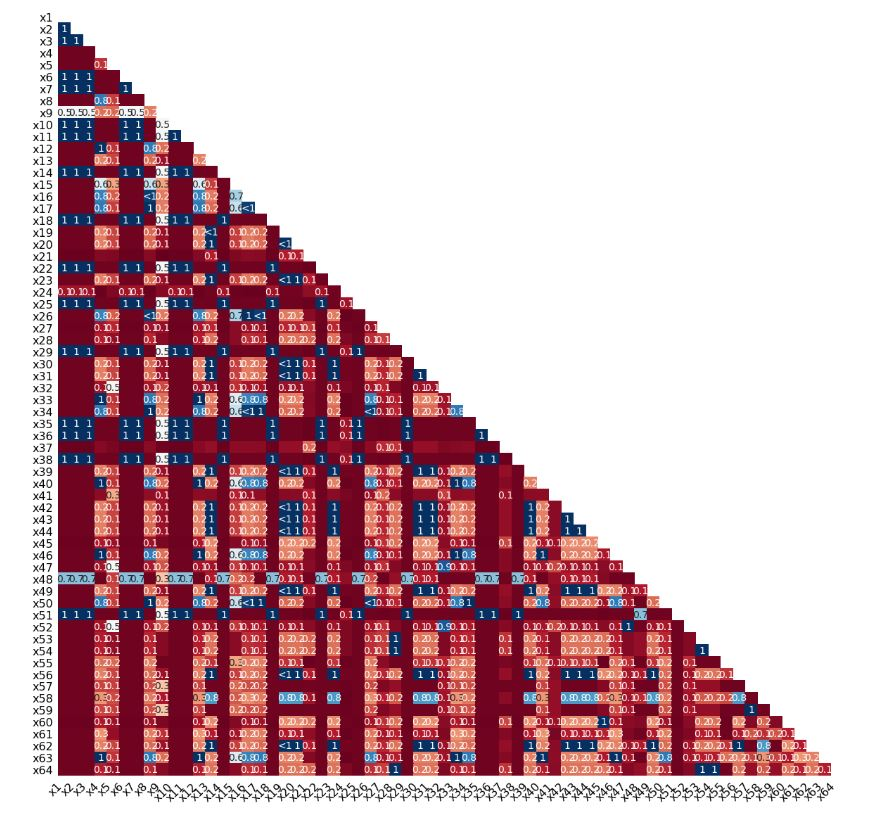
\includegraphics[scale = .6]{imgs/nullity_heatmap.JPG}
  \caption{Nullity Correaltion Heatmap for Year 2 }
  \label{fig:nullity_heatmap}
\end{figure}


